\documentclass[12pt]{article}

\usepackage[fleqn]{amsmath}
\usepackage{amssymb}
\usepackage{amsthm}
\usepackage{graphicx}
\usepackage{float}
\theoremstyle{plain}     %------- 'regular' theorem types
\newtheorem{thm}{Theorem}[section]
\newtheorem{cor}[thm]{Corollary}
\newtheorem{lemma}[thm]{Lemma}
\newtheorem{prop}[thm]{Proposition}
\newtheorem{example}[thm]{Example}
\newtheorem{exer}[thm]{Exercise}
\newtheorem{define}[thm]{Definition}
\usepackage[top=2cm, left=2cm, right=2cm]{geometry} 
\usepackage{parskip}
\setlength{\parindent}{0in}
\usepackage{floatflt}
\usepackage{multicol}
\usepackage{tabu}
\usepackage[hidelinks]{hyperref}
\hypersetup{
	urlcolor=blue}

%%%%%%%%%%%%%%%%%%%%%%
%%%%%%%%%%%%%%%%%%%%%%%
%%%%%%%%%%%%%%%%%%%%%%%%
\begin{document}
\large
%subject
City Semester  \hspace{8cm} Name:\makebox[6cm]{\hrulefill}
\\
%specific topic
Problem Set One \footnote{questions thanks to Lauren Nelson}\\
\normalsize 
%\emph{Complete all work on a separate sheet of paper with exercises clearly labeled and all reasoning and work given.}\\[.5cm]
\emph{Show all work for full credit.}\\
\begin{enumerate}
	\item Visit NYC Independent Budget Office's site: New York By The Numbers--\url{http://ibo.nyc.ny.us/cgi-park2/}\\
	Find one graph/dataset that interests you, prepare a short presentation (1-2 minutes) for the group on why you chose the dataset, what you find interesting about it, and what others may find surprising about it. (Please use the archive links on the right as well so that we can all have different graphs/datasets.)\\
	
	
\begin{figure}[H]
	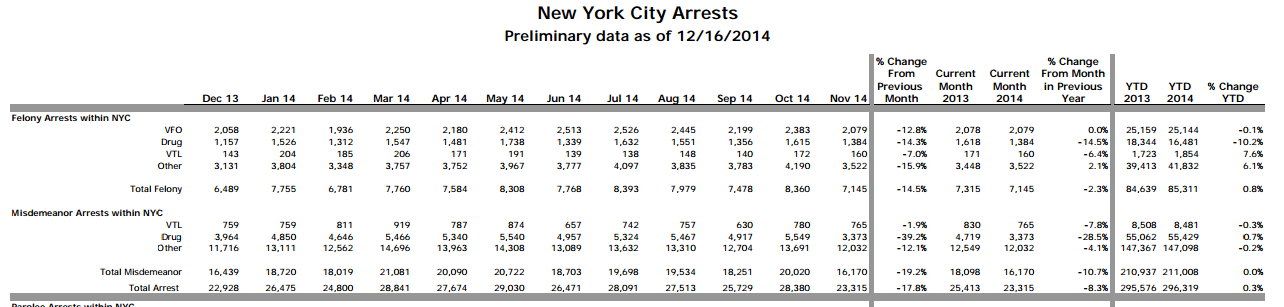
\includegraphics[scale=.4]{1.png}
\end{figure}
	\item How many total arrests were made in NYC from 12/2013 to 11/2014?\\
	\item What percentage of total crimes were felonies?\\
	\item What percentage of July misdemeanor arrests were drug related?\\
	\item Explain what the numbers 0.0\% and -0.1\% in the VFO row mean in the context of the chart and explain how the numbers were calculated.\\
	\item  Do you see any patterns in arrests over the course of the year? Describe.\\
	\item Compare 2014 with 2013. Write a short summary supported by figures from the table that you could imagine being presented as a summation of crime in NYC in 2014.
\newpage	
	\begin{multicols}{2}
		\begin{figure}[H]
			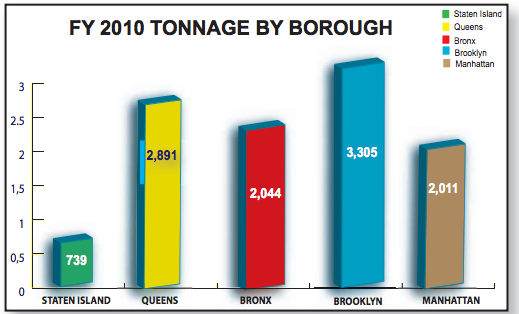
\includegraphics[scale=.4]{2.png}
		\end{figure}
		\begin{figure}[H]
			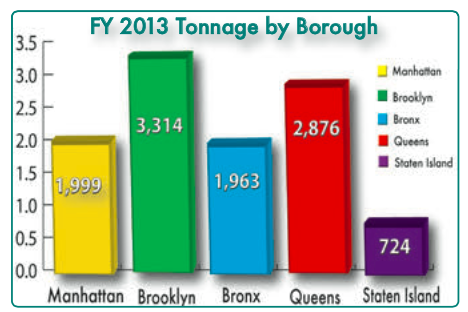
\includegraphics[scale=.4]{3.png}
		\end{figure}
	\end{multicols}
	\item Approximately how many tons of waste were disposed of in all of 2010? What about 2013?\\
	\item What was the percent change from 2010 to 2013 in tons of daily waste per year for each borough?\\
	\item Look up the population of each borough in 2010 (census year). For each borough how much trash was disposed per resident?\\
	\item Look up the geographical area of each borough. How much trash was generated per square foot in 2013? Keep careful track of units.\\
	\item Where does it all go?
	
\end{enumerate}
	
\end{document} 